\documentclass[handout]{beamer}

\usepackage{Haust2017glærur}

\title{Stærðfræðimynstur í tölvunarfræði}
\subtitle{Vika 3, seinni fyrirlestur}

\begin{document}

\begin{frame}
\titlepage
\end{frame}

\section{Inngangur}

\begin{frame}{Í síðasta tíma}
\begin{itemize}
 \item Fylki
 \item Runur og rakningarvensl
 \item Fjöldatölur og reiknanleiki
\end{itemize}
\end{frame}

\section{Skilgreining reiknirits}

\begin{frame}{Vandamál í tölvunarfræði}
\begin{itemize}
 \item Tölvunarfræði felur í sér ýmis vandamál, sum þeirra koma oft fyrir
 \begin{itemize}
  \item Finnum stærstu töluna í þessari runu heiltalna
  \item Tökum þessa runu heiltalna og endurröðum henni í hækkandi röð
  \item Finnum stystu leið á milli þessara tveggja hnúta í neti
 \end{itemize}
 \item Til að tákna vandamálin notum við mengi, runur, föll, net, tré, endanlegar stöðuvélar\ldots
 \item Til að leysa vandamálin notum við \emph{reiknirit}
\end{itemize}
\end{frame}

\begin{frame}{Reiknirit}
Hvað er reiknirit? \pause

Úr bók:
\begin{tcolorbox}[title=Reiknirit]
Reiknirit (e. \emph{algorithm}) er endanleg runa vel skilgreindra aðgerða sem reikna út lausn á skilgreindu vandamáli.
\end{tcolorbox}

\pause
Orðið ``algorithm'' er afleiða latneskunar á nafinu al-Khowarizmi, sem skrifaði um hindú-arabíska talnakerfið. Bók hans, \emph{Kitab al-jabr w'al muquabala}, er þekkt grundvallarrit.

\pause
Orðið kemur fram í \href{https://en.wikipedia.org/wiki/Hauksb\%C3\%B3k}{Hauksbók}!
\end{frame}

\section{Lýsing og eiginleikar reiknirita}

\begin{frame}{Lýsing reiknirita}
Hægt er að nota orð til að lýsa reikniritum. Dæmi úr bók til að finna stærstu heiltölu í runu:

\begin{enumerate}
 \item Set the temporary maximum equal to the first integer in the sequence.
 \item Compare the next integer in the sequence to the temporary maximum, and if it is larger
than the temporary maximum, set the temporary maximum equal to this integer.
 \item Repeat the previous step if there are more integers in the sequence.
 \item Stop when there are no integers left in the sequence. The temporary maximum at this
point is the largest integer in the sequence.
\end{enumerate}
\end{frame}

\begin{frame}{Sauðakóði}
\begin{itemize}
 \item Orðalýsing á reikniritum er oft mjög löng og óþægileg
 \item Til að auðvelda lýsingar nota ýmsir höfundar oft svokallaðan sauðakóða (e. \emph{pseudocode})
 \item Sauðakóði á að vera ``auðveldur aflestrar''
 \begin{itemize}
  \item Í sauðakóða vantar ýmis útfærsluatriði sem algeng eru í forritunarmálum
  \item Í sauðakóða er leyfilegt að lýsa atriðum sem myndu taka margar aðgerðir í tölvu með því að nota setningar
 \end{itemize}
\end{itemize}
\end{frame}

\begin{frame}{Reiknirit með sauðakóða}
Reiknirit sem finnur stærsta stak í runu, sett fram með sauðakóða

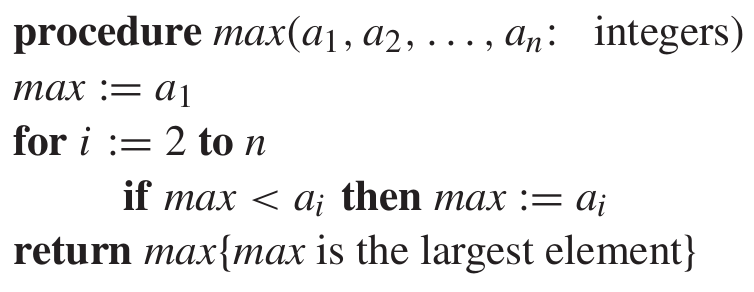
\includegraphics[width=\linewidth]{max-element}
\end{frame}

\begin{frame}{Eiginleikar reiknirita}
    \begin{itemize}
     \item Nokkrir eiginleikar eru flestum reikniritum sameiginlegir
     \item Koma fyrir aftur og aftur í lýsingum reiknirita
     \begin{itemize}
      \item Vandamál sem leysa skal
      \item Inntak (e. \emph{input})
      \begin{itemize}
       \item Reiknirit tekur við gildum úr skilgreindu mengi, gildin eru inntak þess
       \item Inntak reiknirits inniheldur upplýsingar sem viðkoma vandamálinu
      \end{itemize}
      \item Úttak (e. \emph{output})
      \begin{itemize}
       \item Úttak reiknirits tilheyrir skilgreindu mengi
       \item Úttakið lýsir niðurstöðum reikniritsins, sem er lausn á vandamáli
      \end{itemize}
     \end{itemize}
    \end{itemize}
    \end{frame}
    
    \begin{frame}{Fleiri atriði í reikniritalýsingum}
    \begin{itemize}
     \item Fleiri atriði:
     \begin{itemize}
      \item Sé hvert skref reiknirits vel skilgreint og ákvarðanlegt er það skýrt (e. \emph{definite})
      \item Skili reiknirit væntri niðurstöðu fyrir sérhvert inntak er það rétt (e. \emph{correct})
      \item Skili reiknirit niðurstöðu á endanlegum tíma er það endanlegt (e. \emph{finite})
      \item Sé hægt að útfæra hvert skref reikniritsins á endanlegum tíma er það nýtanlegt (e. \emph{effective})
      \item Virki reiknirit á öll tilvik vandamálsins er það almennt (e. \emph{general})
     \end{itemize}
     \item Oftast viljum við að reiknirit hafi alla þessa eiginleika
    \end{itemize}
    \end{frame}

\section{Leitarreiknirit}

\begin{frame}{Leitarreiknirit}
\begin{itemize}
 \item Leit að lið í runu kemur víða við
 \begin{itemize}
  \item Er þessi nemandi í námskeiðinu? 
  \item Er þetta orð rétt skrifað?
 \end{itemize}
 \item Getum skilgreint leitarvandamálið fyrir runur:
 \begin{itemize}
  \item Gefið er $x$ og runa $a_1, a_2, \ldots, a_n$
  \item Þurfum að finna $i$ svo að $x = a_i$ sé það til
  \item Sé slíkt $i$ ekki til segjum við $i = 0$
 \end{itemize}
\end{itemize}
\end{frame}

\begin{frame}{Línuleg leit}
Línuleg leit er reiknirit sem leysir leitarvandamálið fyrir runur:

\begin{center}
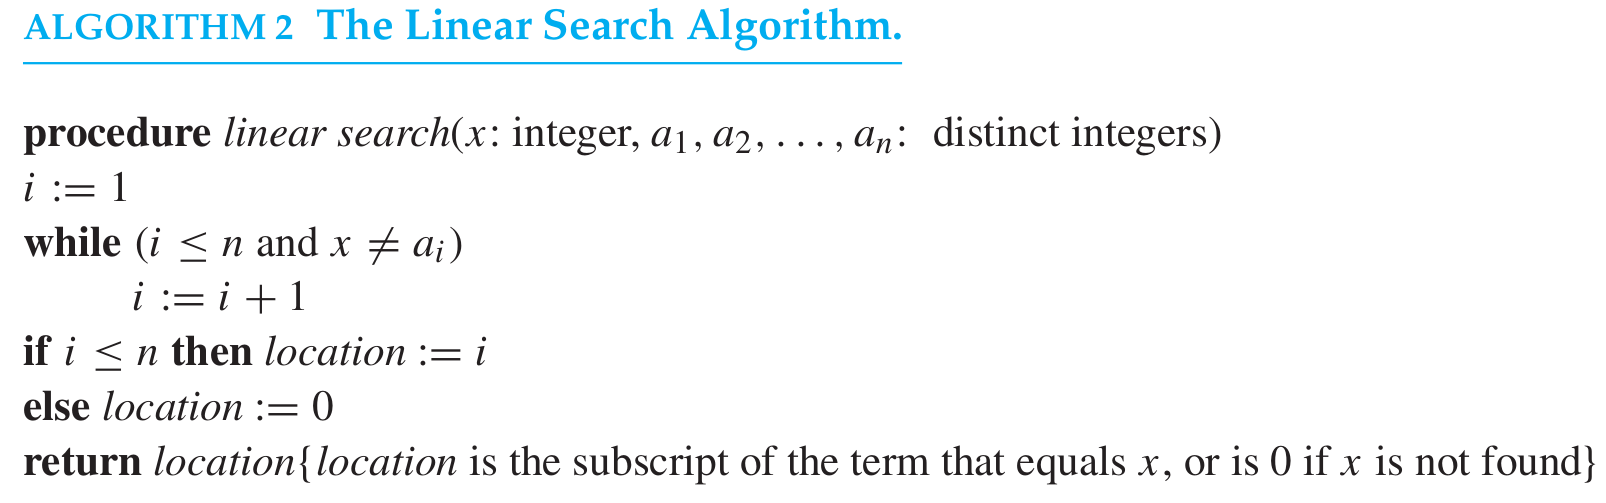
\includegraphics[width=\textwidth]{linear-search}
\end{center}
\end{frame}

\begin{frame}{Getum við gert betur?}
\begin{itemize}
 \item Línuleg leit virkar oft ágætlega
 \begin{itemize}
  \item Hún er einföld
  \item Virkar á allar runur
 \end{itemize}
 \item Ef við vitum meira um rununa getum við oft notað öflugri aðferðir
 \item Ef runan er röðuð getum við notað helmingunarleit
\end{itemize}
\end{frame}

\begin{frame}{Helmingunarleit}
Helmingunarleit er afar skilvirkt leitarreiknirit sem virkar á raðaðar runur.

\begin{center}
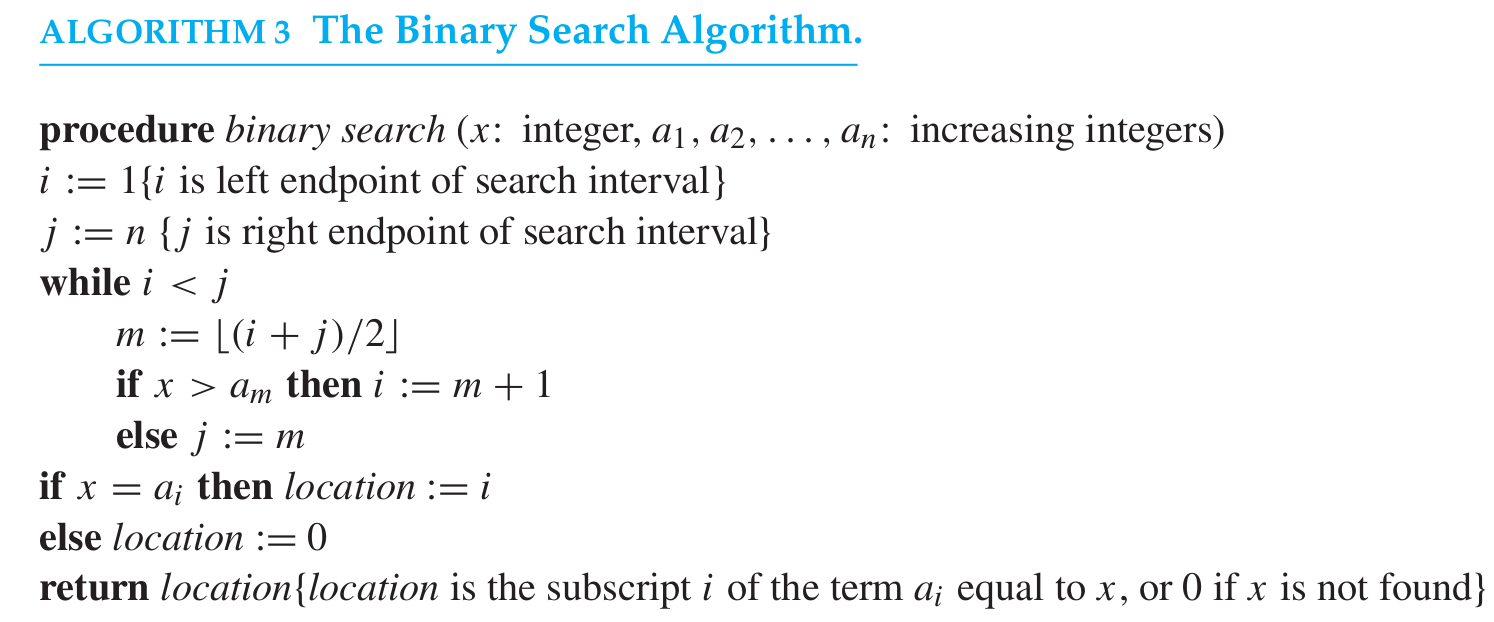
\includegraphics[width=\textwidth]{binary-search}
\end{center}
\end{frame}

\section{Röðunarreiknirit}

\begin{frame}{Röðunarreiknirit}
\begin{itemize}
 \item Annar flokkur vandamála sem oft kemur við sögu er röðunarvandamál
 \begin{itemize}
  \item Búa til orðabók
  \item Setja fram vörulista\ldots
 \end{itemize}
 \item Röðunarvandamálið hefur fengið mikla athygli
 \begin{itemize}
  \item Yfir 100 þekkt reiknirit
  \item $\approx$400 blaðsíður um efnið í \emph{The Art of Computer Programming} eftir Donald Knuth
 \end{itemize}
\end{itemize}
\end{frame}

\begin{frame}{Röðunarvandamálið}
Lausn á röðunarvandamáli fyrir runu talna $a_1, a_2, \ldots, a_n$ felur í sér að finna endurröðun $a'_1, a'_2, \ldots, a'_n$ á rununni svo að $a'_1 \leq a'_2 \leq \ldots \leq a'_n$.
\end{frame}


\begin{frame}{Innsetningarröðun}
\begin{itemize}
 \item Reikniritið innsetningarröðun (e. \emph{insertion sort}) leysir röðunarvandamálið
 \item Lýsing úr bók
 \begin{itemize}
  \item Byrjum að skoða $a_2$, berum það saman við $a_1$
  \begin{itemize}
   \item Sé $a_2 < a_1$ skiptum við á staðsetningum þeirra
   \item Eftir þetta skref eru fyrstu tvö stökin í innbyrðis réttri röð
  \end{itemize}
  \item $a_3$ er borið saman við $a_1$
  \begin{itemize}
   \item Sé það stærra en $a_1$ er það borið saman við $a_2$
   \item Sett á réttan stað í fyrstu þrenndinni
  \end{itemize}
  \item Almennt er stak númer $j$ borið saman við öll $j-1$ stökin sem á undan koma
 \end{itemize}
\end{itemize}
\end{frame}

\begin{frame}{Innsetningarröðun - sauðakóði}
\begin{center}
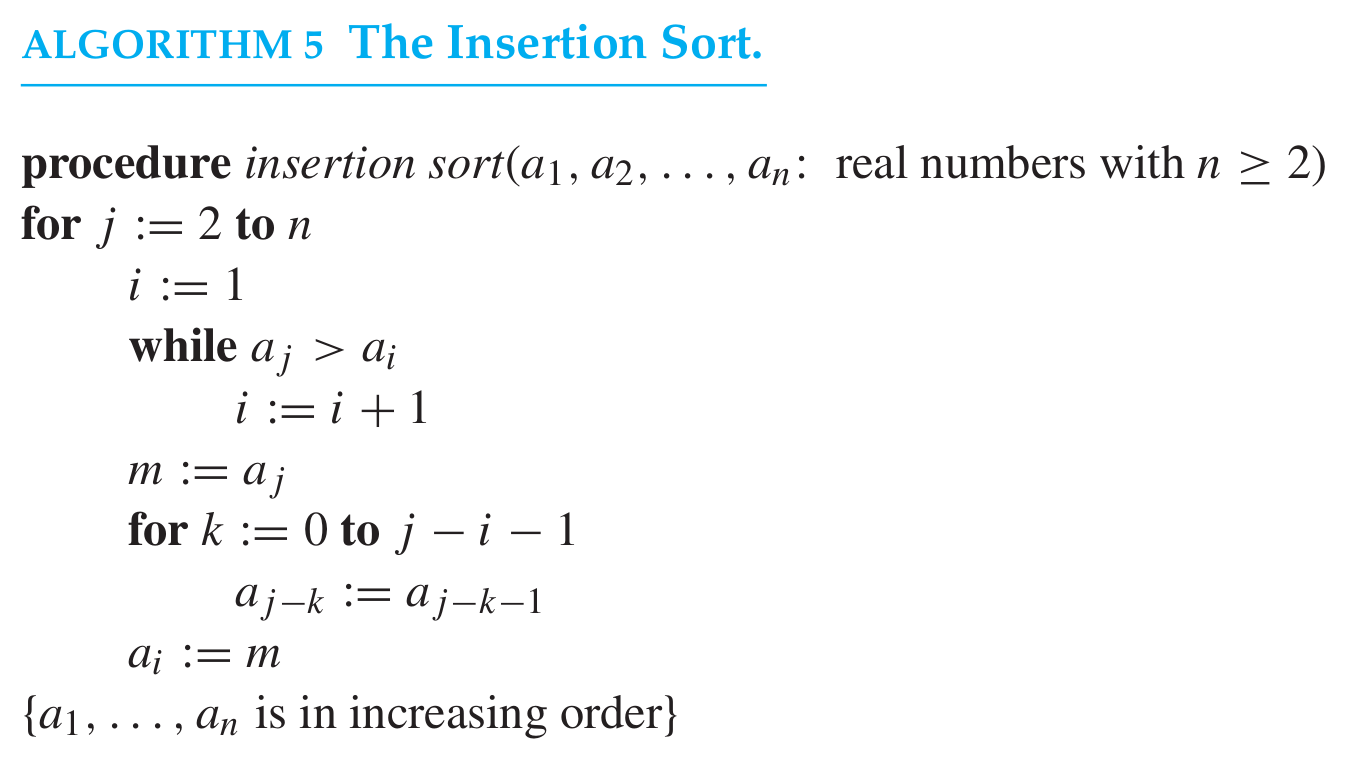
\includegraphics[width=\textwidth]{insertion-sort}
\end{center}
\end{frame}

\section{Gráðug reiknirit}

\begin{frame}{Bestunarreiknirit}
\begin{itemize}
 \item Stór flokkur vandamála sem leysa þarf við raunverulegar aðstæður er bestunarvandamál (e. \emph{optimization problems})
 \item Í bestunarvandamáli höfum við mengi mögulegra lausna, þurfum að finna þá bestu m.t.t. gefins viðmiðs
 \item Einn einfaldasti flokkur reiknirita sem leysir bestunarvandamál er gráðug reiknirit (e. \emph{greedy algorithms})
 \begin{itemize}
  \item Gráðugt reiknirit leysir bestunarvandamál sem skipta má upp í skref með því að velja besta valkostinn í hverju skrefi
  \item Sum gráðug reiknirit finna alltaf bestu lausn með þessum hætti, sum ekki
 \end{itemize}
\end{itemize}
\end{frame}

\begin{frame}{Gráðugt reiknirit fyrir skiptimynt}
\begin{itemize}
 \item Athugum skiptimyntarvandamálið
 \begin{itemize}
  \item Algengt vandamál þangað til á þessari öld \pause
 \end{itemize}
 \item Erum með endanlegan fjölda mismunandi mynta
 \item Viljum rétta manneskju upphæðina $n$
 \item Viljum rétta eins fáar myntir og við getum
 \item Þetta vandamál má leysa á gráðugan máta
\end{itemize}
\end{frame}

\begin{frame}{Gráðug myntskipti}
\begin{itemize}
 \item Gráðug aðferð: Teljum til myntir, í hvert skipti veljum við stærstu mynt $\leq n$
 \begin{itemize}
  \item Drögum verðgildi myntarinnar frá $n$
  \item Veljum aftur stærstu mynt sem ekki er stærri en ``nýja $n$''
  \item Endurtökum
 \end{itemize}
 \item Þessi aðferð skilar stundum bestu lausn, fer eftir verðgildum myntanna
 \begin{itemize}
  \item Alltaf besta lausn fyrir myntgildin $25, 10, 5, 1$
  \item Ekki alltaf besta lausn fyrir myntgildin $25, 10, 1$
 \end{itemize}
\end{itemize}
\end{frame}

\begin{frame}{Gráðug myntskipti}
\begin{center}
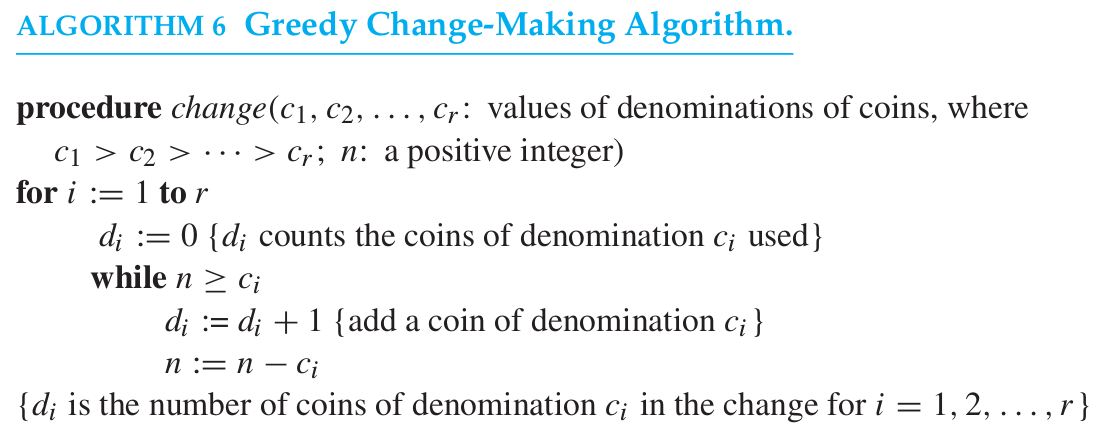
\includegraphics[width=\textwidth]{coin-change}
\end{center}
\end{frame}

\section{Stöðvunarvandamálið}

\begin{frame}{Stöðvunarvandamálið}
\begin{itemize}
 \item Áður hefur verið haldið fram að óákvarðanleg föll séu til
 \item Sýnum nú að til sé vandamál sem ekkert forrit getur leyst
 \item Dæmi um slíkt vandamál er stöðvunarvandamálið (e. \emph{the halting problem})
 \begin{itemize}
  \item Forrit sem leysir stöðvunarvandamálið myndi geta tekið inn annars vegar forrit og hins vegar inntak í forritið og svarað hvort að forritið muni ná að ljúka keyrslu eða ekki 
 \end{itemize}
 \item Alan Turing sýndi að ekki er til forrit sem leysir stöðvunarvandamálið árið 1936
\end{itemize}
\end{frame}

\begin{frame}{Aths. um stöðvunarvandamálið}
    \begin{itemize}
    \item Athugum: Það dugar ekki einfaldlega að keyra forritið $P$ með inntakinu $I$ til að ákvarða vandamálið
    \begin{itemize}
    \item Ef $P$ klárar vitum við vissulega svarið\ldots
    \item \ldots en meðan það er enn að keyra vitum við ekki hvort það mun klára eftir eina sekúndu, eftir milljarð ára eða aldrei
    \end{itemize}
    \item Gerum kröfu um að forritið sé rétt, endanlegt og almennt
    \end{itemize}
\end{frame}

\begin{frame}{Sönnun með mótsögn}
\begin{itemize}
 \item Gerum ráð fyrir að við séum með forrit $H$ sem leysir stöðvunarvandamálið fyrir forrit $P$ og inntak $I$
 \begin{itemize}
  \item $H$ skilar strengnum ``stoppar'' ef $P$ stoppar gefið $I$ sem inntak, annars ``keyrir endalaust'' \pause
 \end{itemize}
 \item Athugum að forrit er safn tákna, svo forrit er strengur, streng má nota sem inntak
 \item Leysi $H$ stöðvunarvandamálið á það því að geta svarað því hvort $P$ stoppar þegar $P$ sjálft er notað sem inntak
\end{itemize}
\end{frame}

\begin{frame}{Sönnun með mótsögn}
\begin{itemize}
 \item Búum nú til forrit $K(P)$ sem notar $H(P, P)$
 \begin{itemize}
  \item Skili $H(P, P)$ strengnum ``keyrir endalaust'' stoppar $K(P)$ 
  \item Skili $H(P, P)$ strengnum ``stoppar'' fer $K(P)$ í endalausa lykkju
  \item $K(P)$ gerir sem sagt það gagnstæða við $H(P, P)$
 \end{itemize}
\end{itemize}
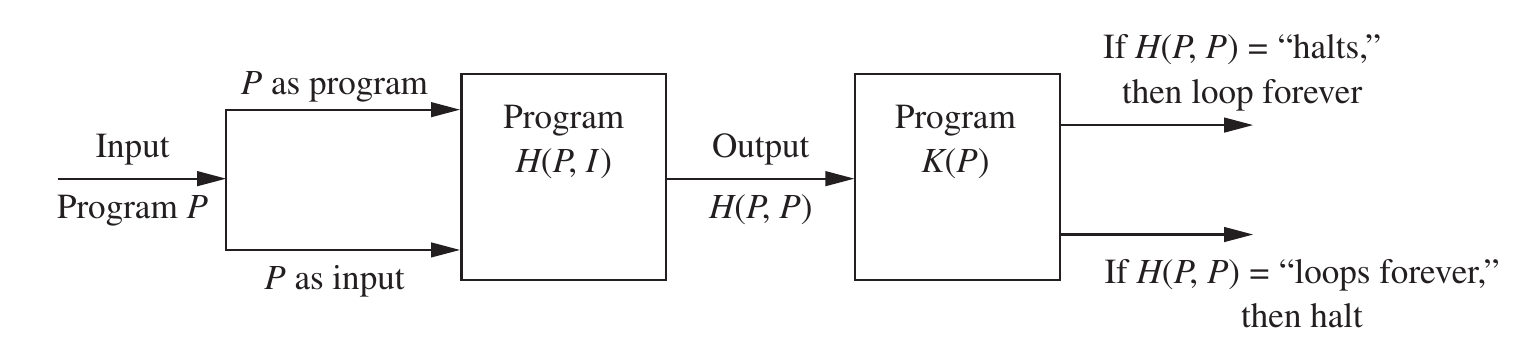
\includegraphics[width=\textwidth]{haltingproblem}

\pause
En hvað gerist ef við köllum á $K(K)$?
\end{frame}

\begin{frame}{Sönnun með mótsögn}
\begin{itemize}
 \item Ef $H(K, K)$ segir að $K(K)$ ljúki keyrslu, þá lýkur $K(K)$ ekki keyrslu
 \item Ef $H(K, K)$ segir að $K(K)$ ljúki ekki keyrslu, þá lýkur $K(K)$ keyrslu
 \item Mótsögn!
 \begin{itemize}
  \item Ekki er til $H$ sem leysir stöðvunarvandamálið fyrir öll forrit
 \end{itemize}
\end{itemize}
\end{frame}

\begin{frame}{Af hverju?}
    \begin{itemize}
        \item Gagnlegt er að vita af óleysanlegum vandamálum
        \item Til að sýna að vandamál sé óleysanlegt dugar að sýna að lausn á því myndi duga til að leysa stöðvunarvandamálið
    \end{itemize}
\end{frame}


\begin{frame}{Næst}
Vöxtur falla (kafli 3.2)
\end{frame}


\end{document}
